\documentclass{beamer}

\usepackage[dutch]{babel}
\usepackage{graphicx}
\usepackage{amsmath}
\usepackage{amssymb}
\usepackage{amsthm}
\usepackage{wasysym}
\usepackage{float}
\usepackage{listings}
\usepackage{setspace}
\usepackage{tikz}
\usepackage{subcaption}
\usepackage{caption}
\usetikzlibrary{arrows}

\AtBeginSection[]{
  \begin{frame}
  \vfill
  \centering
  \begin{beamercolorbox}[sep=8pt,center,shadow=true,rounded=true]{title}
    \usebeamerfont{title}\insertsectionhead\par%
  \end{beamercolorbox}
  \vfill
  \end{frame}
}

\begin{document}

\lstset{language=Haskell}
\title{Individueel project}
\subtitle{Compiler voor een zuiver functionele taal}
\author{Koen Pauwels}
\maketitle

\section{Introductie}

\begin{frame}
  \frametitle{Persoonlijke doelstellingen}
  \begin{itemize}
  \item Niet-triviaal project in Haskell
  \item Beter begrip van werking compiler, ihb lazy evaluation
  \end{itemize}
\end{frame}

\begin{frame}
  \frametitle{Overzicht compiler/interpreter}
  \begin{enumerate}
  \item Gebruiker geeft programma in in verrijkte LC
  \item Programma wordt vertaald naar gewone LC (boomstructuur)
  \item Boomstructuur wordt geherinterpreteerd als graaf
  \item Uitvoering programma door middel van graafreductie
  \end{enumerate}
\end{frame}

\begin{frame}
  \frametitle{Lambdacalculus}
  \begin{enumerate}
  \item Een constante, of
  \item Een variabele, of
  \item Een applicatie van de vorm ``\textless expressie\textgreater \textless expressie\textgreater''.
  \item Een abstractie van de vorm ``$\lambda$ \textless variabele\textgreater .\textless expressie\textgreater''.
  \end{enumerate}
\end{frame}

\begin{frame}
  \frametitle{Verrijkte lambdacalculus}
  \begin{figure}
    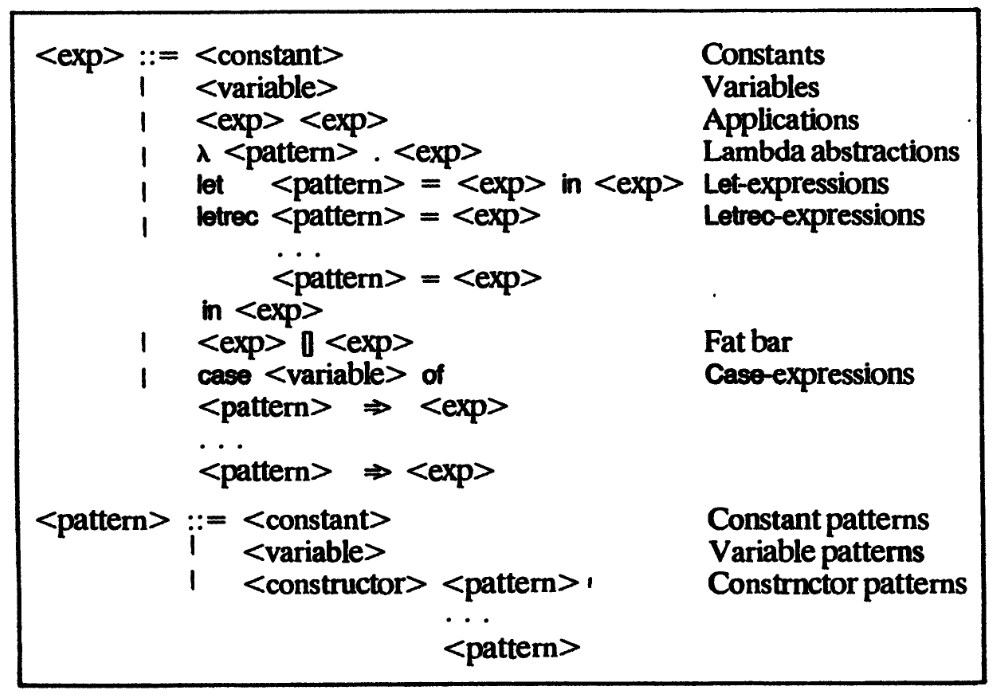
\includegraphics[width=\linewidth]{images/ELC_syntax}
  \end{figure}
\end{frame}

%% ELC -> LC %%%%%%%%%%%%%%%%%%%%%%%%%%%%%%%%%%%%%%%%%%%%%%%%%%%%%%%%%%%%%%%%%%%
\section{Verrijkte lambdacalculus naar lambdacalculus}
\begin{frame}[fragile]
  \frametitle{Voorbeeld onweerlegbaar patroon}
  \begin{lstlisting}
data Pair a b = Pair a b

let second = \(PAIR x y).y
in second (PAIR 1 2)
  \end{lstlisting}
wordt
  \begin{lstlisting}
UNPACK-PRODUCT-PAIR (\x.\y.y)
                    (CONSTR-PAIR 1 2)
  \end{lstlisting}
wat verder wordt uitgewerkt tot
  \begin{lstlisting}
(\x.\y.y) (SEL-PAIR-1 (CONSTR-PAIR 1 2))
          (SEL-PAIR-2 (CONSTR-PAIR 1 2))
  \end{lstlisting}
\end{frame}

\begin{frame}[fragile]
  \frametitle{Voorbeeld weerlegbaar patroon}
  \begin{lstlisting}
data List a = CONS a (List a) | NIL

case x of (CONS x y) -> x; (NIL) -> 0;
  \end{lstlisting}
wordt
  \begin{lstlisting}
(\a. (UNPACK-SUM-CONS (\x.\y.x) a)
     []
     (UNPACK-SUM-NIL a))
x
  \end{lstlisting}
\end{frame}


\begin{frame}[fragile]
  \frametitle{Voorbeeld recursie}
  \begin{lstlisting}
letrec fac = \n . IF (= n 0)
                     1
                     (* n (fac (- n 1)))
in fac 2
  \end{lstlisting}
wordt
  \begin{lstlisting}
(\fac.fac 2) (Y (\n.IF (= n 0)
                    1
                    (* n (- n 1))))
  \end{lstlisting}
\end{frame}


%% REDUCTIE %%%%%%%%%%%%%%%%%%%%%%%%%%%%%%%%%%%%%%%%%%%%%%%%%%%%%%%%%%%%%%%%%%%%
\section{Reductie}

\begin{frame}[fragile]
  \frametitle{Reductie: waarom een graaf?}
  \begin{lstlisting}
(\x.AND x x) (NOT TRUE)
-> AND (NOT TRUE) (NOT TRUE)
-> AND FALSE (NOT TRUE)
-> AND FALSE FALSE
-> FALSE
  \end{lstlisting}
\end{frame}

\begin{frame}
  \frametitle{Reductie: waarom een graaf?}
  \begin{figure}
    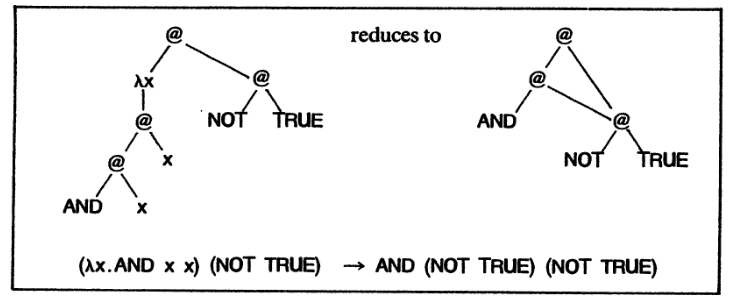
\includegraphics[width=\linewidth]{images/slpj208}
  \end{figure}
\end{frame}

\begin{frame}
  \frametitle{Implementatie van de graaf}
  \begin{figure}
    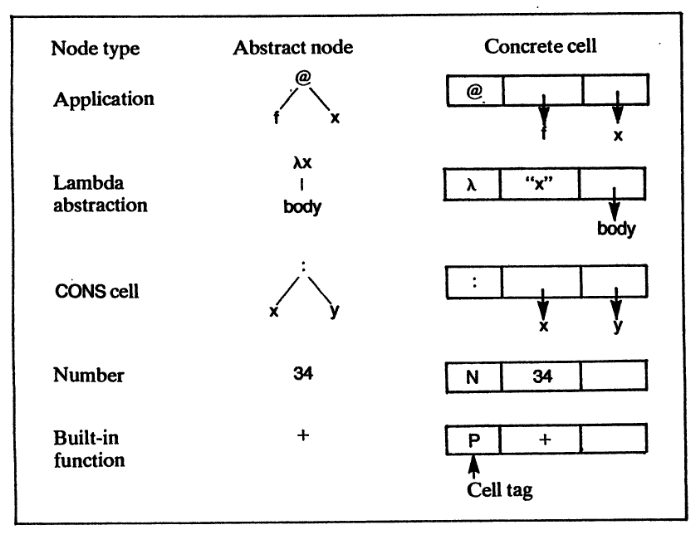
\includegraphics[width=\linewidth]{images/cells}
  \end{figure}
\end{frame}

\begin{frame}
  \frametitle{Reductie gedreven door nood om output te produceren}
  \begin{enumerate}
  \item Printing mechanisme roept reduce functie aanknopingspunt op.
  \item Die reduceert de graaf tot die zich in \emph{weak head normal form (WHNF)} bevindt.
  \item Als het resultaat een lijst is, gaat het printing mechanisme zichzelf recursief oproepen eerst op het eerste element van de lijst, en dan op de rest van de lijst. Anders wordt het resultaat onmiddellijk uitgeprint en is de huidige call van de print procedure klaar.
\end{enumerate}
\end{frame}

\begin{frame}
  \frametitle{Hoe de volgende redex te vinden}
  \begin{figure}[h]
    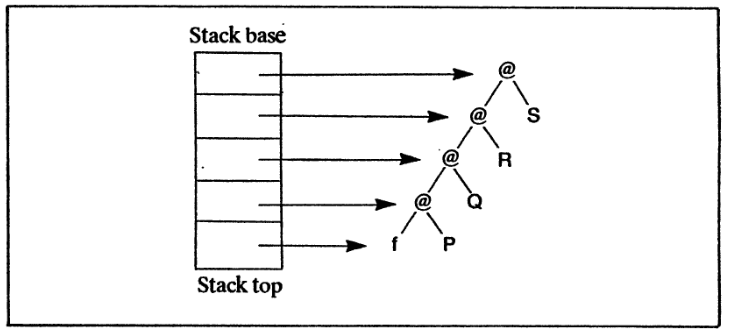
\includegraphics[width=\linewidth]{images/slpj203}
    \caption{Illustratie van de spine stack (f P Q R S)}
  \end{figure}
\end{frame}

\begin{frame}
  \frametitle{Hoe de volgende redex te vinden}
  \begin{figure}
    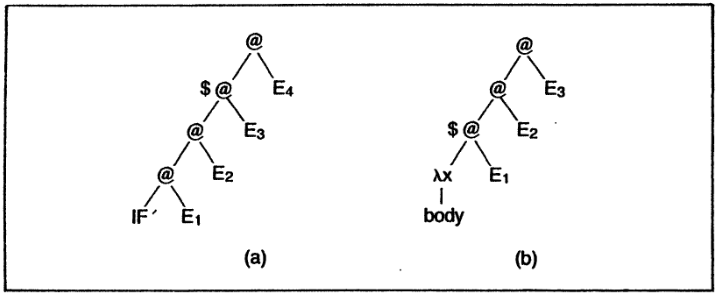
\includegraphics[width=\linewidth]{images/slpj202}
    \caption{Voorbeelden van redex selectie (redex gemarkeerd met '\$')}
  \end{figure}
\end{frame}

\end{document}
